\documentclass{standalone}

\usepackage{tikz}
\usetikzlibrary{circuits.ee.IEC}
\usetikzlibrary{positioning}

\usepackage[compatibility, RPvoltages]{circuitikz}
\ctikzset{bipoles/length=.9cm}

\begin{document}
 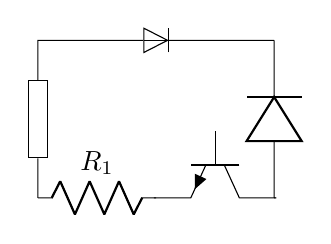
\begin{tikzpicture}[circuit ee IEC]
  \draw (0,0) to [resistor={name=R}] (0,2)
	to[diode={name=D}] (3,2);
  \draw (0,0) to[*R=$R_1$] (1.5,0) to[*Tnpn] (3,0)
    to[*D](3,2);
 \end{tikzpicture}
\end{document}
